\documentclass[10pt,twocolumn]{article}
\usepackage[a4paper,margin=0.62in,columnsep=0.24in]{geometry}
\usepackage[T1]{fontenc}
\usepackage{times}
\usepackage{microtype}
\usepackage{booktabs,tabularx,array}
\usepackage{enumitem}
\usepackage{titlesec}
\usepackage{amsmath}
\usepackage{float}
\usepackage{xcolor}
\usepackage{tikz}
\usetikzlibrary{positioning,arrows.meta}
\usepackage[hidelinks]{hyperref}

\titleformat{\section}{\normalsize\bfseries}{\thesection}{0.5em}{}
\titlespacing*{\section}{0pt}{6pt}{2pt}
\titleformat{\subsection}{\small\bfseries}{\thesubsection}{0.5em}{}
\titlespacing*{\subsection}{0pt}{4pt}{1pt}
\setlist{nosep,leftmargin=1.1em}
\setlength{\parskip}{2pt}
\setlength{\parindent}{0pt}
\raggedbottom
\renewcommand{\arraystretch}{1.05}
\newcolumntype{Y}{>{\raggedright\arraybackslash}X}

\begin{document}
\twocolumn[{
\begin{center}
{\Large\bfseries Knowing When Not to Answer: Abstention Drift in\\[2pt] Multi-Turn Retrieval-Augmented Conversations}\\[5pt]
{\small CS683 Natural Language Processing \,\textbullet\, Initial Project Report}\\[3pt]
{\small Team: \textit{Member 1} \,\textbullet\, \textit{Member 2} \,\textbullet\, \textit{Member 3} \,\textbullet\, \textit{Member 4} \,\textbullet\, \textit{Member 5}}
\end{center}
\vspace{4pt}
}]

\section{Problem Statement}
Retrieval-augmented generation (RAG) assistants are widely deployed as conversational agents, but they often answer confidently even when the retrieved documents do not contain the answer. In the SemEval-2026 multi-turn RAG task (MTRAGEval), one of the strongest systems reached 83.9\% answerability accuracy yet detected only \textbf{21.8\% of unanswerable turns} \cite{ails}: its LLM judges favoured plausible-sounding answers over evidence. Research on abstention (a model declining to answer) is almost entirely single-turn \cite{wen2025,feng}, while real conversations get longer and more context-dependent as they go on. We ask:

\textbf{RQ1.} Does detection of unanswerable questions get worse at later turns in a conversation (\emph{abstention drift})?\\
\textbf{RQ2.} Can a lightweight answerability checker, trained on cheaply generated unanswerable examples, reduce this drift \emph{without} increasing wrong refusals on answerable turns?

\section{Datasets}
We use the \textbf{MTRAG} benchmark family (Apache-2.0), which also serves as the data for SemEval-2026 Task~8.

\textbf{MTRAG} \cite{mtrag} (TACL 2025): 110 human-written conversations (avg.\ 7.7 turns) converted to 842 tasks. Each task is one turn with its full history, a reference answer, human-labelled reference passages, and an answerability label (709 answerable, 68 partial, 55 unanswerable, 10 conversational). There are four domains: ClapNQ (Wikipedia), Cloud (technical documentation), FiQA (finance forums) and Govt (government web pages). Their passage-level corpora total about 366K passages. Human-written standalone rewrites of each question are also provided, and we use them as an upper bound for query rewriting. \emph{Use:} train/dev, split 80/20 \emph{by conversation} to avoid leakage.

\textbf{MTRAG-UN} \cite{mtragun} (Findings ACL 2026): the SemEval-2026 evaluation benchmark, focused on UNanswerable, UNderspecified and non-standalone questions. The 507 publicly released tasks (285 answerable, 47 partial, 97 unanswerable, 78 underspecified) use the same four corpora. \emph{Use:} held-out test set.

\begin{table}[H]
\centering\small
\begin{tabular}{@{}lccc@{}}
\toprule
\% unanswerable & Turns 1--2 & Turns 3--5 & Turns 6+ \\
\midrule
MTRAG (842 tasks) & 5.0 & 6.8 & 7.4 \\
MTRAG-UN (507 tasks) & 9.4 & 13.8 & 33.7 \\
\bottomrule
\end{tabular}
\caption{\small Share of unanswerable tasks by turn position (our analysis of the released data).}
\label{tab:data}
\end{table}
\vspace{-10pt}
Table~\ref{tab:data} shows that unanswerable questions cluster in late turns. A raw comparison across turns is therefore \emph{confounded}, and our method controls for this (\S3.3).

\begin{table*}[t]
\centering\footnotesize
\begin{tabularx}{\textwidth}{@{}p{1.25cm}p{2.3cm}Yp{4.1cm}@{}}
\toprule
\textbf{Member} & \textbf{Role} & \textbf{Responsibilities} & \textbf{Key deliverable (week)} \\
\midrule
Member 1 & Retrieval lead & Corpus indexing (BM25, BGE, FAISS), reciprocal rank fusion, cross-encoder re-ranking, retrieval recall@5/nDCG, retrieval ablations & Indexes for 4 domains (W1); S1--S2 retrieval (W2) \\
Member 2 & Generation \& rewriting & LLM query rewriting, grounded-answer and refusal prompts, running S0--S4, official MTRAG answer-quality evaluation & S0 baseline (W1); S0--S4 predictions (W3) \\
Member 3 & Checker \& data & Evidence-removal synthesis and filters, DeBERTa-v3 checker training, threshold selection under the false-abstention budget & Synthetic data (W2); trained S3/S4 checkers (W2--W3) \\
Member 4 & Evaluation \& analysis & Per-turn metrics, drift slope with bootstrap CIs, controlled regression, synthetic probe, plots, error analysis & Evaluation script (W1); results tables and plots (W3--W4) \\
Member 5 & Validation, demo \& documentation & Novelty check of SemEval-2026 papers, 50-example human check of synthetic labels, Gradio demo, README, report and slide integration & Novelty memo (W1); demo (W3); report and slides (W4) \\
\bottomrule
\end{tabularx}
\caption{\small Division of work. All members contribute to the final report and presentation.}
\label{tab:work}
\end{table*}

\section{Proposed Method}
\subsection{Pipeline}
\begin{center}
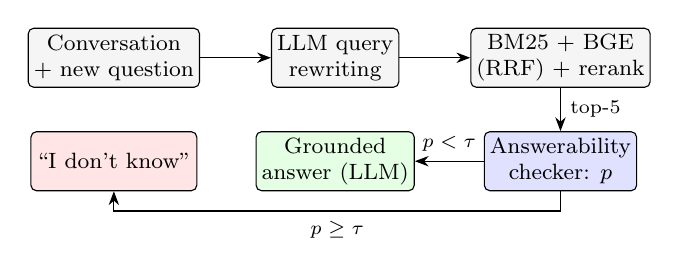
\begin{tikzpicture}[node distance=0.3cm and 0.9cm, every node/.style={font=\footnotesize, align=center}, box/.style={draw, rounded corners=2pt, fill=gray!8, minimum height=0.75cm, minimum width=1.6cm, inner sep=2pt}, ar/.style={-{Stealth[length=5pt]}}]
\node[box] (a) {Conversation\\+ new question};
\node[box, right=of a] (b) {LLM query\\rewriting};
\node[box, right=of b] (c) {BM25 + BGE\\(RRF) + rerank};
\node[box, below=0.55cm of c, fill=blue!12] (d) {Answerability\\checker: $p$};
\node[box, below=0.55cm of b, fill=green!10] (e) {Grounded\\answer (LLM)};
\node[box, below=0.55cm of a, fill=red!10] (f) {``I don't know''};
\draw[ar] (a)--(b); \draw[ar] (b)--(c); \draw[ar] (c)--node[right,font=\scriptsize]{top-5}(d);
\draw[ar] (d)--node[above,font=\scriptsize]{$p<\tau$}(e);
\draw[ar] (d.south) -- ++(0,-0.25) -| node[pos=0.25,below,font=\scriptsize]{$p\ge\tau$} (f.south);
\end{tikzpicture}
\end{center}
\begin{enumerate}
\item \textbf{Query rewriting:} an instruction-tuned LLM (Qwen2.5-3B/7B, 4-bit) turns each follow-up question into a standalone query.
\item \textbf{Hybrid retrieval:} BM25 and dense BGE-small \cite{bge} results are merged with reciprocal rank fusion \cite{rrf}, then re-ranked by a BGE cross-encoder (top-5 passages).
\item \textbf{Answerability checker (our contribution):} a DeBERTa-v3-base \cite{deberta} cross-encoder reads the query and the top-5 passages and outputs $p=P(\text{unanswerable})$. If $p\ge\tau$ the system replies ``I don't know''; otherwise the LLM answers only from the passages.
\end{enumerate}

\subsection{Evidence removal: free unanswerable data}
Only 6.5\% of MTRAG turns are unanswerable, too few to train on. For every \emph{answerable} turn we know which passages hold the answer. Re-running retrieval while excluding \emph{all} passages from those source documents gives a realistic context that no longer supports the answer, producing a new unanswerable example at no annotation cost. Answerable examples are also built from retrieval (with the gold passages inserted), so the checker cannot learn a ``gold passages look different'' shortcut. We drop generated examples whose passages still cover the reference answer (a word-overlap filter plus an optional LLM check), and we hand-check 50 kept examples to report label noise. The threshold $\tau$ maximises abstention F1 subject to refusing $\le$5\% of answerable dev turns (RQ2).

\subsection{Evaluation}
\textbf{Abstention quality:} precision, recall and F1 on unanswerable turns, and the false-abstention rate on answerable turns, per turn bucket (1--2, 3--5, 6+). \textbf{Abstention drift} is the slope $\beta$ of $P(\text{abstain}\mid\text{unanswerable})$ against turn number $t$:
\[
\Pr[\hat a_i=1] = \alpha + \beta\, t_i ,\qquad y_i=\text{UNANSWERABLE}
\]
with a 95\% CI from a bootstrap that resamples whole conversations. To separate turn position from question type, we (i) fit a logistic regression controlling for domain and follow-up type, and (ii) run a \emph{synthetic probe}: evidence removal applied at every turn position of the dev conversations, so only the passages change. \textbf{Answer quality:} official MTRAG metrics (ROUGE-L, BERTScore, LLM-judge faithfulness).

\textbf{Systems compared:} S0 last-turn query + BM25 + prompt-only refusal; S1 + LLM rewriting; S2 + hybrid retrieval and re-ranking; S3 = S2 + checker trained on real labels only; \textbf{S4} = S2 + checker trained on real + synthetic data (proposed); S4-oracle uses human rewrites (upper bound).

\section{Novelty over Prior Work}
MTRAG and MTRAG-UN \cite{mtrag,mtragun} report unanswerable performance as a single aggregate number, and SemEval-2026 systems focus on leaderboard scores \cite{ails}. Abstention studies \cite{wen2025,feng} evaluate isolated questions. To our knowledge, no prior work (i) measures how abstention changes with \emph{turn position} while controlling for question type, or (ii) creates unanswerable training data for conversational RAG by removing evidence documents. Both are cheap to run, reusable, and directly relevant to deployed assistants.

\section{Deliverables}
\begin{itemize}
\item Public GitHub repository: modular code, configuration files, unit tests, reproducible scripts (a starter version with 14 passing tests exists).
\item Trained answerability checker, prediction files for S0--S4 in the official MTRAG format, and a hand-checked sample of 50 synthetic examples.
\item Results: per-turn abstention tables, drift slopes with CIs, a drift plot, ablations and error analysis.
\item Interactive Gradio demo that shows sources and a $P(\text{unanswerable})$ meter.
\item Final 2-page report and presentation slides; if results are strong, an extended short paper for an ACL Rolling Review cycle.
\end{itemize}

\section{Division of Work (5 members, 4 weeks)}
Each member owns one component end to end and one week-by-week deliverable (Table~\ref{tab:work}); every member reviews one other member's code through pull requests.

\textbf{Timeline.} W1: data, indexes, S0 baseline, evaluation script, novelty check. W2: rewriting and hybrid retrieval (S1--S2), synthetic data, checker training (S3--S4). W3: MTRAG-UN runs, drift analysis, synthetic probe, demo. W4: error analysis, final report and slides.

\section{Risks and Mitigation}
\begin{itemize}
\item \textbf{Prior work on per-turn abstention appears:} checked in week~1. Fallback: study the acceptance bias of LLM answerability judges \cite{ails} with the same pipeline.
\item \textbf{Noisy synthetic labels} (another document still answers): lexical and LLM filters, a 50-example human check, and the threshold tuned only on real dev data.
\item \textbf{Few real unanswerables} (55 + 97): conversation-level bootstrap CIs, plus the synthetic probe for statistical power.
\item \textbf{Limited compute:} 4-bit 3B model locally (GTX 1650, 4\,GB); final 7B runs on free Kaggle/Colab GPUs.
\end{itemize}

\section{Expected Outcomes}
(i) A quantified answer to RQ1: whether, and by how much, abstention recall drops per extra turn, with the confound from question position controlled. (ii) Evidence for RQ2: whether synthetic evidence-removed data improves unanswerable recall over prompt-only refusal (S2) and real-label training (S3) at a fixed 5\% false-abstention budget. (iii) A reusable open-source toolkit and demo.

{\footnotesize
\begin{thebibliography}{9}\setlength{\itemsep}{0pt}
\bibitem{mtrag} Y.~Katsis, S.~Rosenthal, et al. MTRAG: A Multi-Turn Conversational Benchmark for Evaluating RAG Systems. \emph{TACL} 13:784--808, 2025.
\bibitem{mtragun} S.~Rosenthal, Y.~Katsis, et al. MTRAG-UN: A Benchmark for Open Challenges in Multi-Turn RAG Conversations. \emph{Findings of ACL}, 2026.
\bibitem{ails} D.~Athanasiou et al. AILS-NTUA at SemEval-2026 Task 8: Multi-Turn RAG Conversations. \emph{SemEval}, 2026. arXiv:2603.10524.
\bibitem{wen2025} B.~Wen et al. Know Your Limits: A Survey of Abstention in Large Language Models. \emph{TACL}, 2025.
\bibitem{feng} S.~Feng et al. Don't Hallucinate, Abstain: Identifying LLM Knowledge Gaps via Multi-LLM Collaboration. \emph{ACL}, 2024.
\bibitem{rrf} G.~Cormack, C.~Clarke, S.~B\"uttcher. Reciprocal Rank Fusion Outperforms Condorcet and Individual Rank Learning Methods. \emph{SIGIR}, 2009.
\bibitem{bge} S.~Xiao et al. C-Pack: Packed Resources for General Chinese Embeddings. \emph{SIGIR}, 2024.
\bibitem{deberta} P.~He, J.~Gao, W.~Chen. DeBERTaV3: Improving DeBERTa using ELECTRA-Style Pre-Training with Gradient-Disentangled Embedding Sharing. \emph{ICLR}, 2023.
\end{thebibliography}}
\end{document}
